\chapter{Results}
\begin{comment}


\end{comment}

\section{Results from the Lenard-Jones Potential with direct Summation}
\begin{comment}

\end{comment}

% Plot of the total energy as a function of time
\begin{figure}
	\begin{center}
		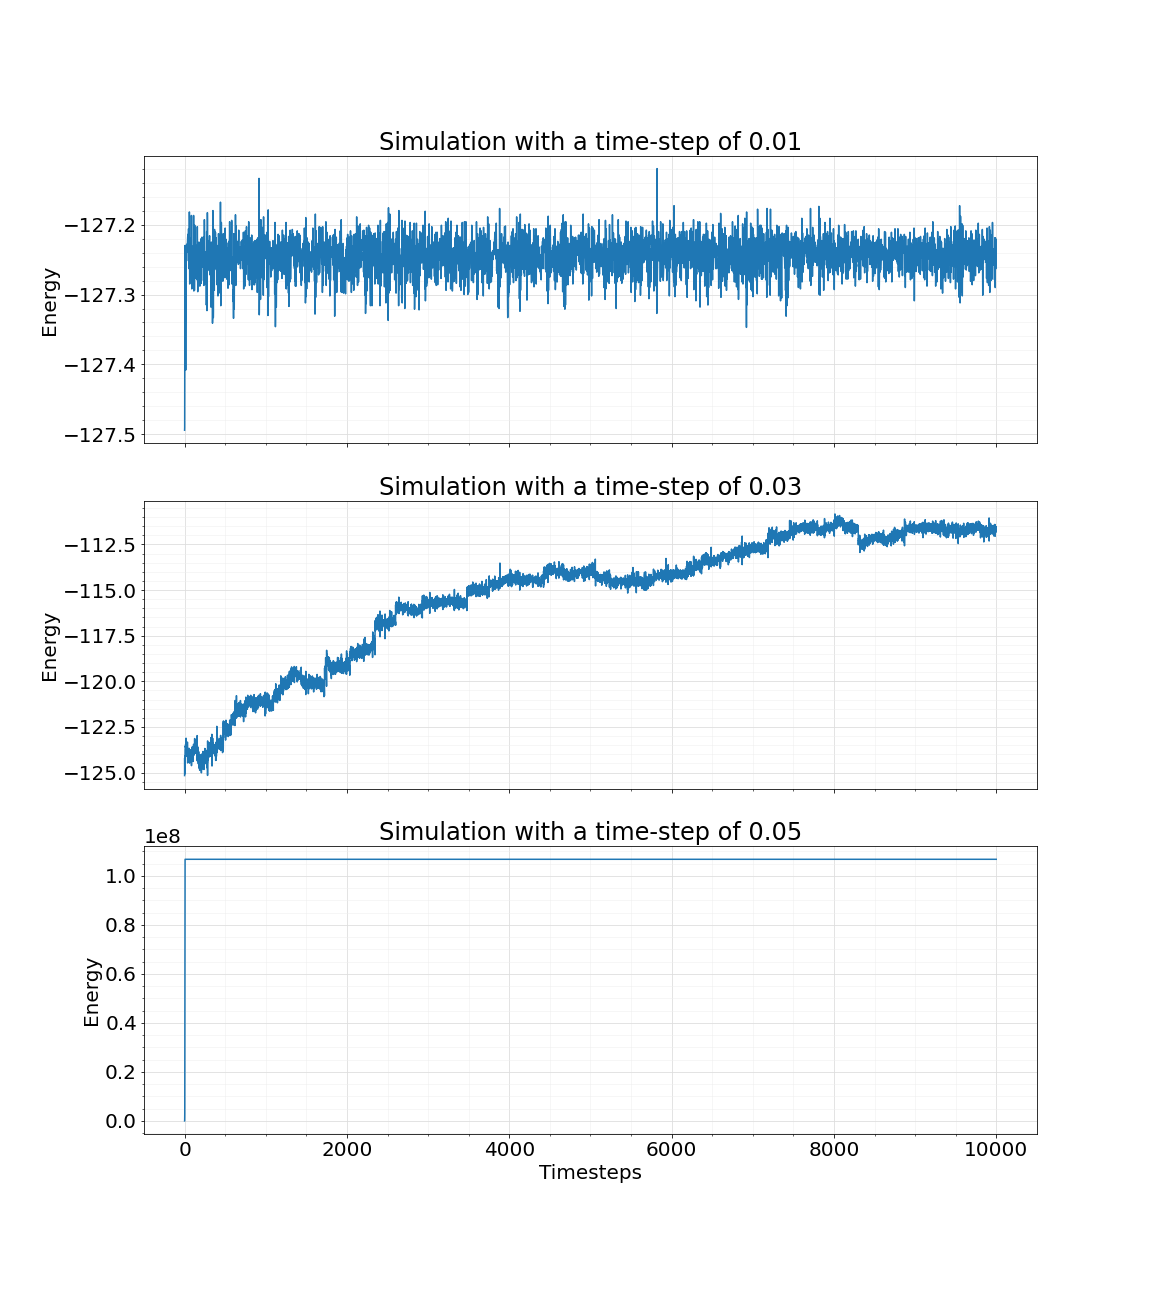
\includegraphics[scale= 1.05]{/home/cm/CLionProjects/MDCode/AData//totalEnergyDrift.png}
	\end{center}
	\caption[Simulation with different timesteps]{Simulation with different timesteps}
	\label{SimWithTimestep}
\end{figure}
The first task of the course asks to plot the total energy of the simulation for different time steps. The units were in a Lenard-Jones equivalent and not given here. As can be seen in the sequence \ref{SimWithTimestep}, with a bigger and bigger timestep the energy in the simulation goes from stable (timestep 0.01) over a drifting behavior (timestep 0.03) to being unstable (timestep 0.05). A good timestep for this simulation would be 0.01.  
\par
To visualize the simulation OVITO \cite{ovito} was used and this series of images was created.
% Simulation Snapshots
\begin{figure}
	\begin{center}
		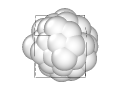
\includegraphics[scale= 0.65]{Figure/1ImageS.png}
	\end{center}
	\caption[Simulation Snapshot]{Simulation Snapshot}
	\label{SimulationSnapshot1}
\end{figure}

\begin{figure}
	\begin{center}
		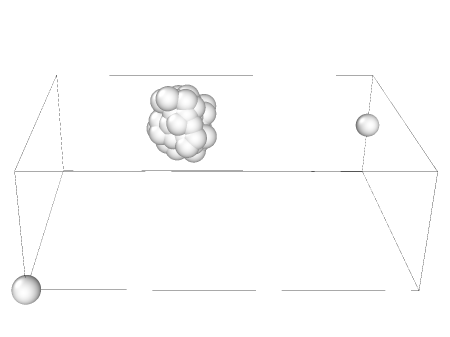
\includegraphics[scale= 0.75]{Figure/2ImageS.png}
	\end{center}
	\caption[Simulation Snapshot]{Simulation Snapshot }
	\label{SimulationSnapshot2}
\end{figure}

\begin{figure}
	\begin{center}
		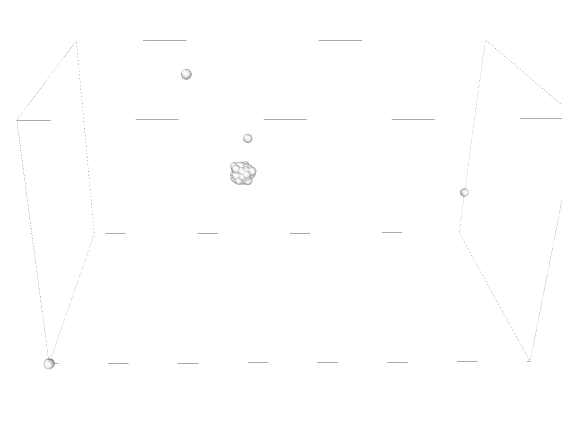
\includegraphics[scale= 0.65]{Figure/3ImageS.png}
	\end{center}
	\caption[Simulation Snapshot]{Simulation Snapshot }
	\label{SimulationSnapshot3}
\end{figure}
As it can be seen in the images \ref{SimulationSnapshot1}, \ref{SimulationSnapshot2} and \ref{SimulationSnapshot3} the Atoms are initially ordered into a blob, which was given in the course. 
Later in the simulation some of the atoms escape the initial blob and fly outward separately. 
\section{Result from the Simulation with the Berendsen Thermostat}
\begin{comment}

\end{comment}


\begin{figure}[!h]
	\begin{center}
		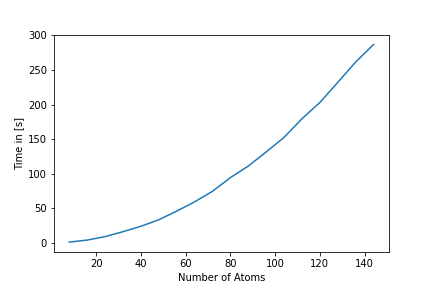
\includegraphics[scale=1]{Figure/plotAtomTimes.png}
	\end{center}
	\caption[Simulationtime with the Berendsen Thermostat from 8 to 192 Atoms]{Simulationtime with the Berendsen Thermostat from 8 to 192 Atoms }
	\label{PlotSimulationTimeBerendsenThermostat}
\end{figure}


\section{Results from the Simulation with the Neighborhood-List}
\begin{comment}

\end{comment}

\begin{figure}[!h]
	\begin{center}
		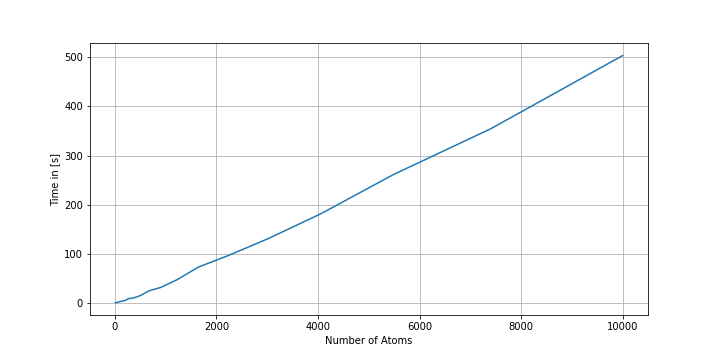
\includegraphics[scale=1.25]{Figure/plotAtomTimesMoreData.png}
	\end{center}
	\caption[Simulationtime with the Neighborhood-list]{Simulationtime with the Neighborhood-list}
	\label{PlotSimulationTimesCutoffNew}
\end{figure}

\section{Results from the Simulation with the Gupta-Potential}
\begin{comment}

\end{comment}

\begin{figure}[!h] 
	\begin{center} 
		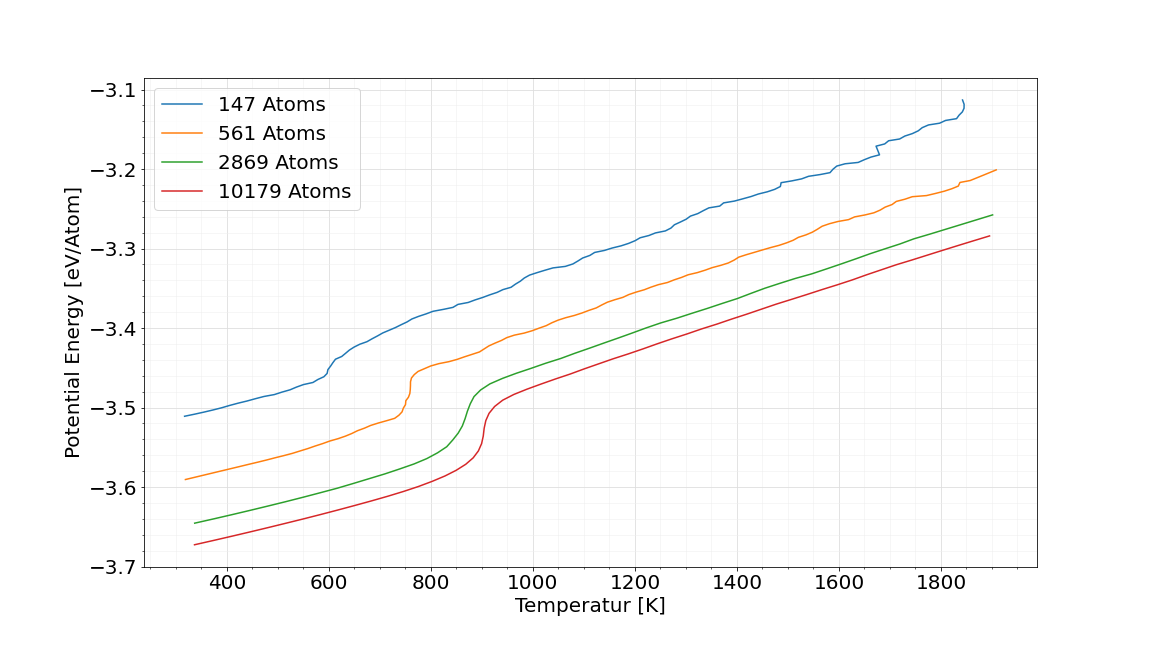
\includegraphics[scale=1.15]{/home/cm/CLionProjects/MDCode/AData/Clusters/temperaturPotentialEnergyCurveMoreInOne.png} 
	\end{center} 
	\caption[Gold Cluster Simulation]{Gold Cluster Simulation} 
	\label{GoldClusterSimulationTemperaturEnergy4In1} 
\end{figure} 

\begin{figure}[!h] 
	\begin{center} 
		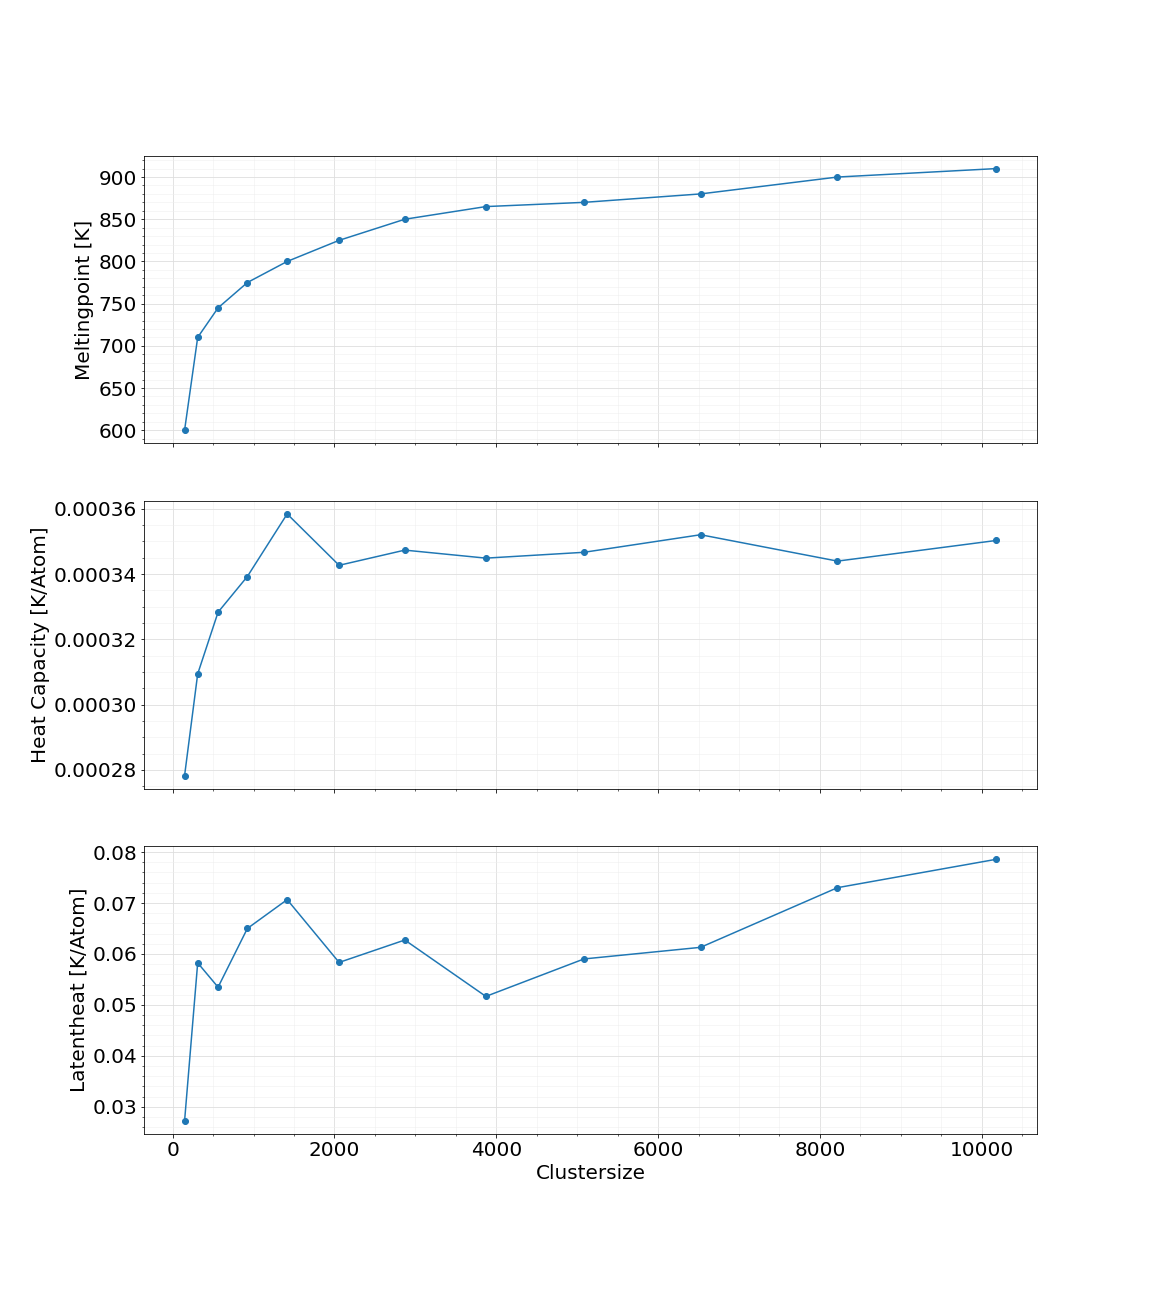
\includegraphics[scale=1.15]{/home/cm/CLionProjects/MDCode/AData/Clusters/VsClusterSizeAll.png} 
	\end{center} 
	\caption[Melting Point, Heat Capacity and Latent Heat vs Clustersize]{Melting Point, Heat Capacity and Latent Heat vs Clustersize} 
	\label{GoldClusterSimulationVsClustersize} 
\end{figure} 
